Ao longo da história do país, o desenvolvimento econômico e social esteve profundamente enraizado em atividades agrícolas e pecuárias \cite{garcao2015pecuaria}. De acordo com a Associação Brasileira das Indústrias Exportadoras de Carnes (ABIEC) \cite{abiec}, o complexo agroindustrial voltado à produção de carne bovina representa cerca de 8,4\% do Produto Interno Bruto (PIB) nacional. Além disso, o Brasil possui o maior rebanho bovino comercial do mundo, correspondendo a 11,6\% do total mundial, e ocupa a primeira posição no comércio exterior de carne bovina, sendo responsável por aproximadamente 21\% da carne negociada internacionalmente \cite{embrapa2}.

Nesse cenário, a avaliação precisa das características da carcaça dos animais desempenha um papel crucial para a cadeia produtiva. Entre os métodos disponíveis, a ultrassonografia se destaca por possibilitar o exame \textit{in vivo}, de forma rápida, com boa precisão e custos relativamente baixos \cite{cap3:medidaAol}. Por meio de imagens de ultrassom, é possível mensurar características como a Área de Olho de Lombo (AOL), a Espessura de Gordura no Lombo (EGL) e a Espessura de Gordura na Garupa (EGG), indicadores diretamente relacionados à musculosidade, precocidade de terminação e qualidade da carne \cite{cap3:carcaça}, localizadas nas regiões de Olho do Lombo (contra-filé), entre a 12ª e a 13ª costela (AOL e EGL) e Garupa (EGG), medida no começo do músculo \textit{Bicips Femolis} (ponta da picanha). A Figura \ref{intro:medidas} mostra uma ilustração da localização das medidas no animal.
\begin{figure}[htpb]
    \centering
    \caption{Ilustração da localização das regiões de interesse.}
    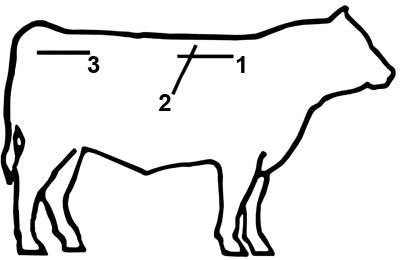
\includegraphics[width = 0.5\linewidth]{figures/introducao/medidas.jpeg}
    \caption*{\footnotesize Fonte: Adaptado de \cite{AgroParanaUltrassom}.}
    \label{intro:medidas}
\end{figure}
A linha horizontal (1) indica a localização da Gordura no lombo onde é possível medir a EGL, a linha vertical (2) indica a localização do Olho do Lombo onde é possível medir a AOL e a linha horizontal (3) indica a localização da Garupa onde é possível medir a EGG. Nestas regiões, as imagens de ultrassom obtidas são mostradas na Figura \ref{intro:ultrasom}.

\begin{figure}[htpb]
    \centering
    \caption{Imagens de ultrassom das regiões de interesse.}
    \begin{subfigure}{0.5\linewidth}
        \centering
        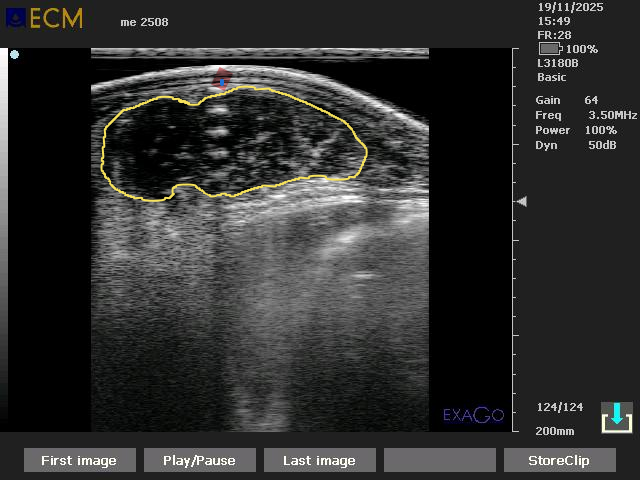
\includegraphics[width=\linewidth]{figures/AOL.png}
        \caption{AOL e EGL.}
    \end{subfigure}
    \hspace{30mm}
    \begin{subfigure}{0.5\linewidth}
        \centering
        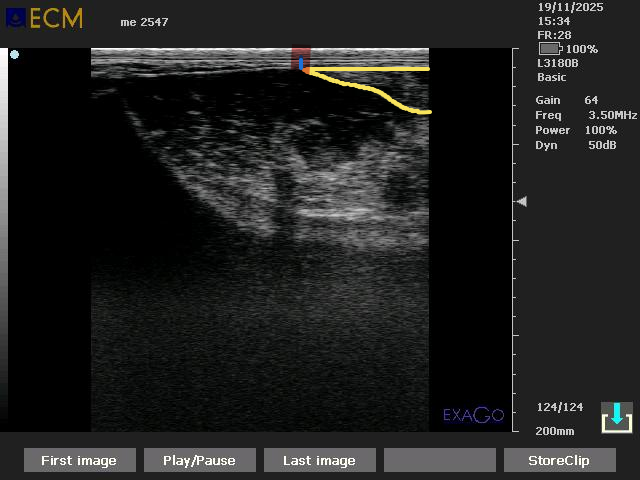
\includegraphics[width=\linewidth]{figures/cap3/medidaEGG.png  }
        \caption{EGG.}

    \end{subfigure}
    \caption*{\footnotesize Fonte: Elaboração do Autor.}
    \label{intro:ultrasom}
\end{figure}
A região dentro da delimitação amarela na Figura \ref{intro:ultrasom} (a) corresponde à AOL, a linha azul dentro da delimitação vermelha, logo acima, indica a localização da EGL. A região dentro da delimitação vermelha, linha azul, na Figura \ref{intro:ultrasom} (b) corresponde à EGG, sendo o \textit{biceps femoris} a demarcação amarela. A variabilidade nessas características influencia a comercialização e os resultados econômicos dos produtores \cite{cap3:nelore_caracu}, tornando sua mensuração precisa uma demanda constante do setor.

Tradicionalmente, a análise dessas imagens de ultrassom e a demarcação das regiões de interesse são realizadas manualmente por especialistas, um processo sujeito à subjetividade e que demanda tempo considerável. Diante disso, a aplicação de técnicas de visão computacional e inteligência artificial \cite{szeliski2010} apresenta-se como uma alternativa promissora para automatizar e padronizar esse processo de mensuração. Em particular, arquiteturas de redes neurais convolucionais (\textit{Convolutional Neural Networks} - CNNs) \cite{cnn}, uma subárea da inteligência artificial dedicada à análise e interpretação de imagens, têm demonstrado resultados expressivos em diversas aplicações biomédicas \cite{Goodfellow-et-al-2016}. Uma das principais técnicas empregadas nessas redes é a segmentação de imagens, que consiste em classificar cada pixel em uma categoria específica, possibilitando a identificação precisa das regiões de interesse. A Figura \ref{intro:segmentacao} ilustra o processo de segmentação.
\begin{figure}[H]
    \centering
    \caption{Exemplo de segmentação de uma imagem de ultrassom.}
    \begin{subfigure}{0.3\linewidth}
        \centering
        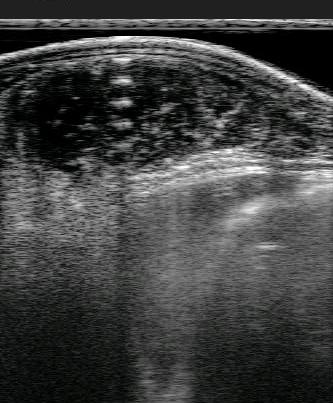
\includegraphics[width=\linewidth]{figures/introducao/ultrasom.jpg}
        \caption{Imagem original.}
    \end{subfigure}
    \hspace{30mm}
    \begin{subfigure}{0.3\linewidth}
        \centering
        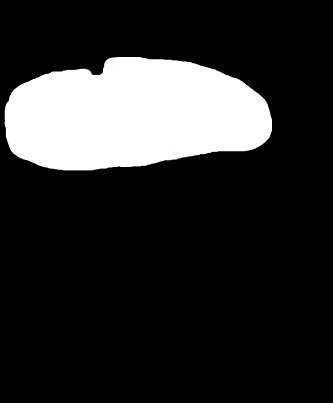
\includegraphics[width=\linewidth]{figures/introducao/segmentacao.jpg }
        \caption{Imagem segmentada.}

    \end{subfigure}
    \caption*{\footnotesize Fonte: Elaboração do Autor.}
    \label{intro:segmentacao}
\end{figure}
A imagem original, Figura \ref{intro:segmentacao} (a), a região de interesse não está demarcada, podendo ser visível apenas por um especialista, enquanto na imagem segmentada, Figura \ref{intro:segmentacao} (b), a região de interesse foi identificada e destacada, facilitando a extração das medidas de AOL (área branca).

Entre as arquiteturas de segmentação, a U-Net\footnote{O nome U-Net vem do formato da arquitetura da rede, que se assemelha à letra U.} \cite{Ronneberger2015UNet} se destaca como principal referência. Trata-se de uma arquitetura \textit{encoder-decoder}: o  \textit{encoder} e a etapa que extrai características progressivamente abstratas da imagem, enquanto o \textit{decoder} as utiliza para reconstruir a segmentação. Originalmente proposta para segmentação de imagens biomédicas, a U-Net é reconhecida pela capacidade de operar com conjuntos de dados reduzidos e pela eficiência na captura de informações contextuais e de detalhes finos das imagens. Quando é necessário que a arquitetura faça algo além da segmentação, como por exemplo, segmentação e classificação, utiliza-se uma abordagem denominada \textit{Multitask} (Multitarefa). Essa abordagem permite que a rede aprenda a realizar múltiplas tarefas simultaneamente, compartilhando representações e melhorando o desempenho geral do modelo. Paralelamente, a teoria dos conjuntos fuzzy \cite{zadeh1965fuzzy} oferece ferramentas para o tratamento de incertezas e imprecisões inerentes a imagens de ultrassom, onde as fronteiras entre as estruturas anatômicas nem sempre são claramente definidas. A integração de redes neurais com a teoria dos conjuntos fuzzy \cite{intro:unetfuzzy}, por meio do Sistema de Inferência Neuro-Fuzzy Adaptativo (ANFIS), possibilita combinar a capacidade de aprendizado das redes neurais com a flexibilidade de um sistema baseado em regras fuzzy (SBRF) no tratamento de informações imprecisas. Alguns estudos têm explorado a aplicação da U-Net em tarefas de segmentação de imagens ultrassom da região de olho de lombo \cite{JadersonMelo2022UNetpp} e sua junção com a teoria dos conjuntos fuzzy \cite{Korshunova2018}.

Neste contexto, este trabalho tem como objetivo desenvolver e comparar dois modelos de segmentação de imagens de ultrassom de bovinos das raças Nelore e Caracu: 
\begin{itemize}
    \item Uma rede U-Net com abordagem \textit{Multitask};
    \item Uma U-Net \textit{Multitask} com a integração do ANFIS. 
\end{itemize}

Foram utilizadas 135 imagens de ultrassom obtidas de animais vivos, localizados no Centro Avançado de Pesquisa Tecnológica do Agronegócio (CAPTA) em Sertãozinho-SP, por meio do aparelho de ultrassom Aloka SSD-500. O intuito é avaliar a precisão e a eficiência dos modelos propostos na segmentação automática das regiões do olho de lombo e da garupa, viabilizando a obtenção automatizada das medidas de AOL, EGL e EGG. Por conta do número limitado de imagens disponíveis, foi necessário realizar um processo de aumento de dados (\textit{data augmentation}) para ampliar o conjunto de treinamento e melhorar a generalização dos modelos. O processo de aumento de dados incluiu técnicas como rotação e adição de ruído às imagens originais, simulando variações que podem ocorrer durante a aquisição das imagens de ultrassom.  Para essa avaliação, utilizam-se quatro métricas: 
\begin{itemize}
    \item O coeficiente de Dice \cite{dice},que quantifica a similaridade entre a imagem segmentada pelo modelo e a imagem de
referência demarcada pelo especialista.
    \item Erro Médio Absoluto (\textit{Mean Absolute Error} -- MAE), que compara as medidas extraídas da imagem segmentada com as medidas obtidas pelo especialista. 
    \item Acurácia, que avalia a capacidade do modelo em classificar corretamente as regiões de interesse.
    \item $R^2$, que mede a proporção da variância explicada pelo modelo em relação à variância total.
\end{itemize}
Foram treinadas duas redes neurais para cada medida, uma com fuzzy e outra sem e foi feito uma correlação cruzada, que consiste em treinar cada modelo uma quantidade de vezes, para avaliar a consistência dos resultados. Neste caso, cada modelo foi treinado quatro vezes. A figura \ref{intro:fluxo} apresenta o fluxo de treinamento e comparação dos modelos propostos, assim como a divisão do banco de dados em conjuntos de treinamento, validação e teste.
\begin{figure}[htpb]
    \centering
    \caption{Fluxo de treinamento e comparação dos modelos propostos para a obtenção das medidas de AOL, EGL e EGG.}
    
\includegraphics[width = 0.6\linewidth]{figures/introducao/fluxo.png}
    \caption*{\footnotesize Fonte: Elaboração do Autor.}
    \label{intro:fluxo}
\end{figure}

Com isso, pretende-se não apenas automatizar a segmentação das imagens de ultrassom, mas também desenvolver um aplicativo que calcule as medidas de AOL, EGL e EGG a partir de novas imagens de ultrassom, tornando a tecnologia acessível para produtores e profissionais do setor agropecuário.

Para alcançar o objetivo, o presente trabalho está organizado da seguinte forma. No Capítulo 1, são apresentados os conceitos fundamentais de redes neurais, desde a inspiração biológica do neurônio artificial até as arquiteturas de redes neurais convolucionais. O Capítulo 2 introduz a teoria dos conjuntos fuzzy e os sistemas baseados em regras fuzzy, que fornecem a base teórica para a construção do ANFIS. O Capítulo 3 descreve detalhadamente a implementação dos modelos propostos, incluindo a arquitetura da U-Net, a integração do ANFIS e o processo de treinamento. O Capítulo 4 apresenta a organização do conjunto de dados, o treinamento e os resultados obtidos, com uma análise comparativa entre os modelos. Por fim, o Capítulo 5 conclui o trabalho, explicando o desenvolvimento do aplicativo, destacando as contribuições e sugerindo direções para pesquisas futuras. 
